\section{Simulation Analysis and Comparison with Theoretical Results}
\label{sec:simulation}


\subsection{Operating Point}

\subsection{Gain}


\begin{figure}[H]
\centering
\begin{subfigure}{.5\textwidth}
    \centering
    \vspace{2.8 cm}
    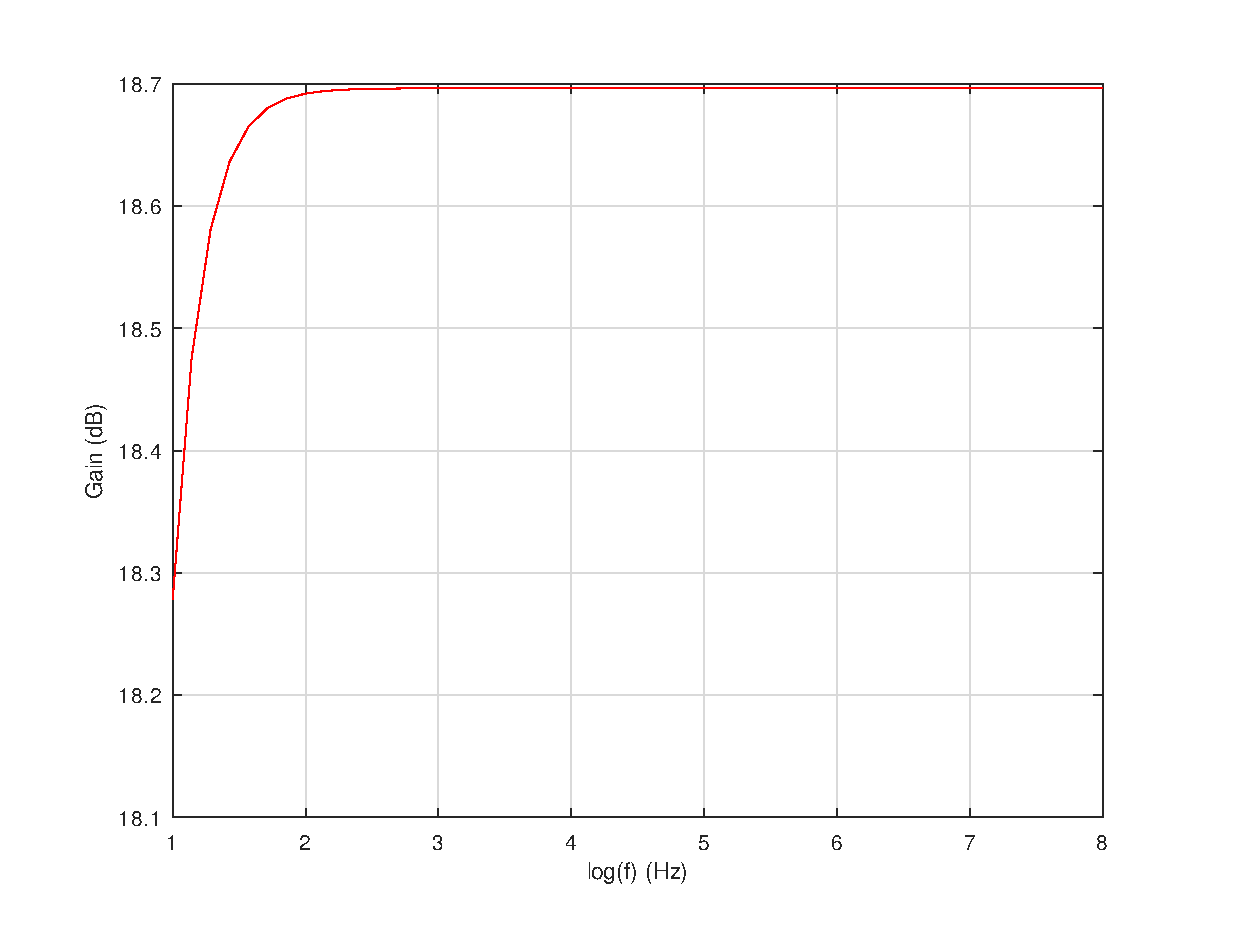
\includegraphics[scale=0.4]{Gain.eps}
    \caption{Theoretical}
\end{subfigure}
\begin{subfigure}{.4\textwidth}
    \centering
    \includegraphics[scale=0.3]{gain.pdf}
    \caption{Simulation}
\end{subfigure}
\caption{Gain}
\label{fig:Gain}
\end{figure}



\subsection{Impedances}


\subsection{Operating Point}
\begin{table}[H]
  \centering
  \begin{tabular}{|l|r|}
    \hline    
    {\bf Formula} & {\bf Merit} \\ \hline
    @c[i] & 0.000000e+00\\ \hline
@gb[i] & -2.24935e-04\\ \hline
@r1[i] & 2.149178e-04\\ \hline
@r2[i] & -2.24935e-04\\ \hline
@r3[i] & -1.00169e-05\\ \hline
@r4[i] & 1.233378e-03\\ \hline
@r5[i] & -2.24935e-04\\ \hline
@r6[i] & 1.018460e-03\\ \hline
@r7[i] & 1.018460e-03\\ \hline
v1 & 5.248421e+00\\ \hline
v2 & 5.033187e+00\\ \hline
v3 & 4.581562e+00\\ \hline
v4 & -2.05008e+00\\ \hline
v5 & 5.064367e+00\\ \hline
v6 & 5.745178e+00\\ \hline
v7 & -2.05008e+00\\ \hline
v8 & -3.09813e+00\\ \hline

  \end{tabular}
  \caption{LEGENDA}
  \label{tab:op}
\end{table}

\begin{table}[H]
  \centering
  \begin{tabular}{|l|r|}
    \hline    
    {\bf Formula} & {\bf Merit} \\ \hline
    zin & 2.236262e+00\\ \hline

  \end{tabular}
  \caption{LEGENDA}
  \label{tab: input}
\end{table}








\begin{figure}[H] \centering
\includegraphics[width=0.4\linewidth]{gain2.pdf}
\caption{LLLLLLLLLLLLLLLLL}
\label{fig:2}
\end{figure}

\begin{figure}[H] \centering
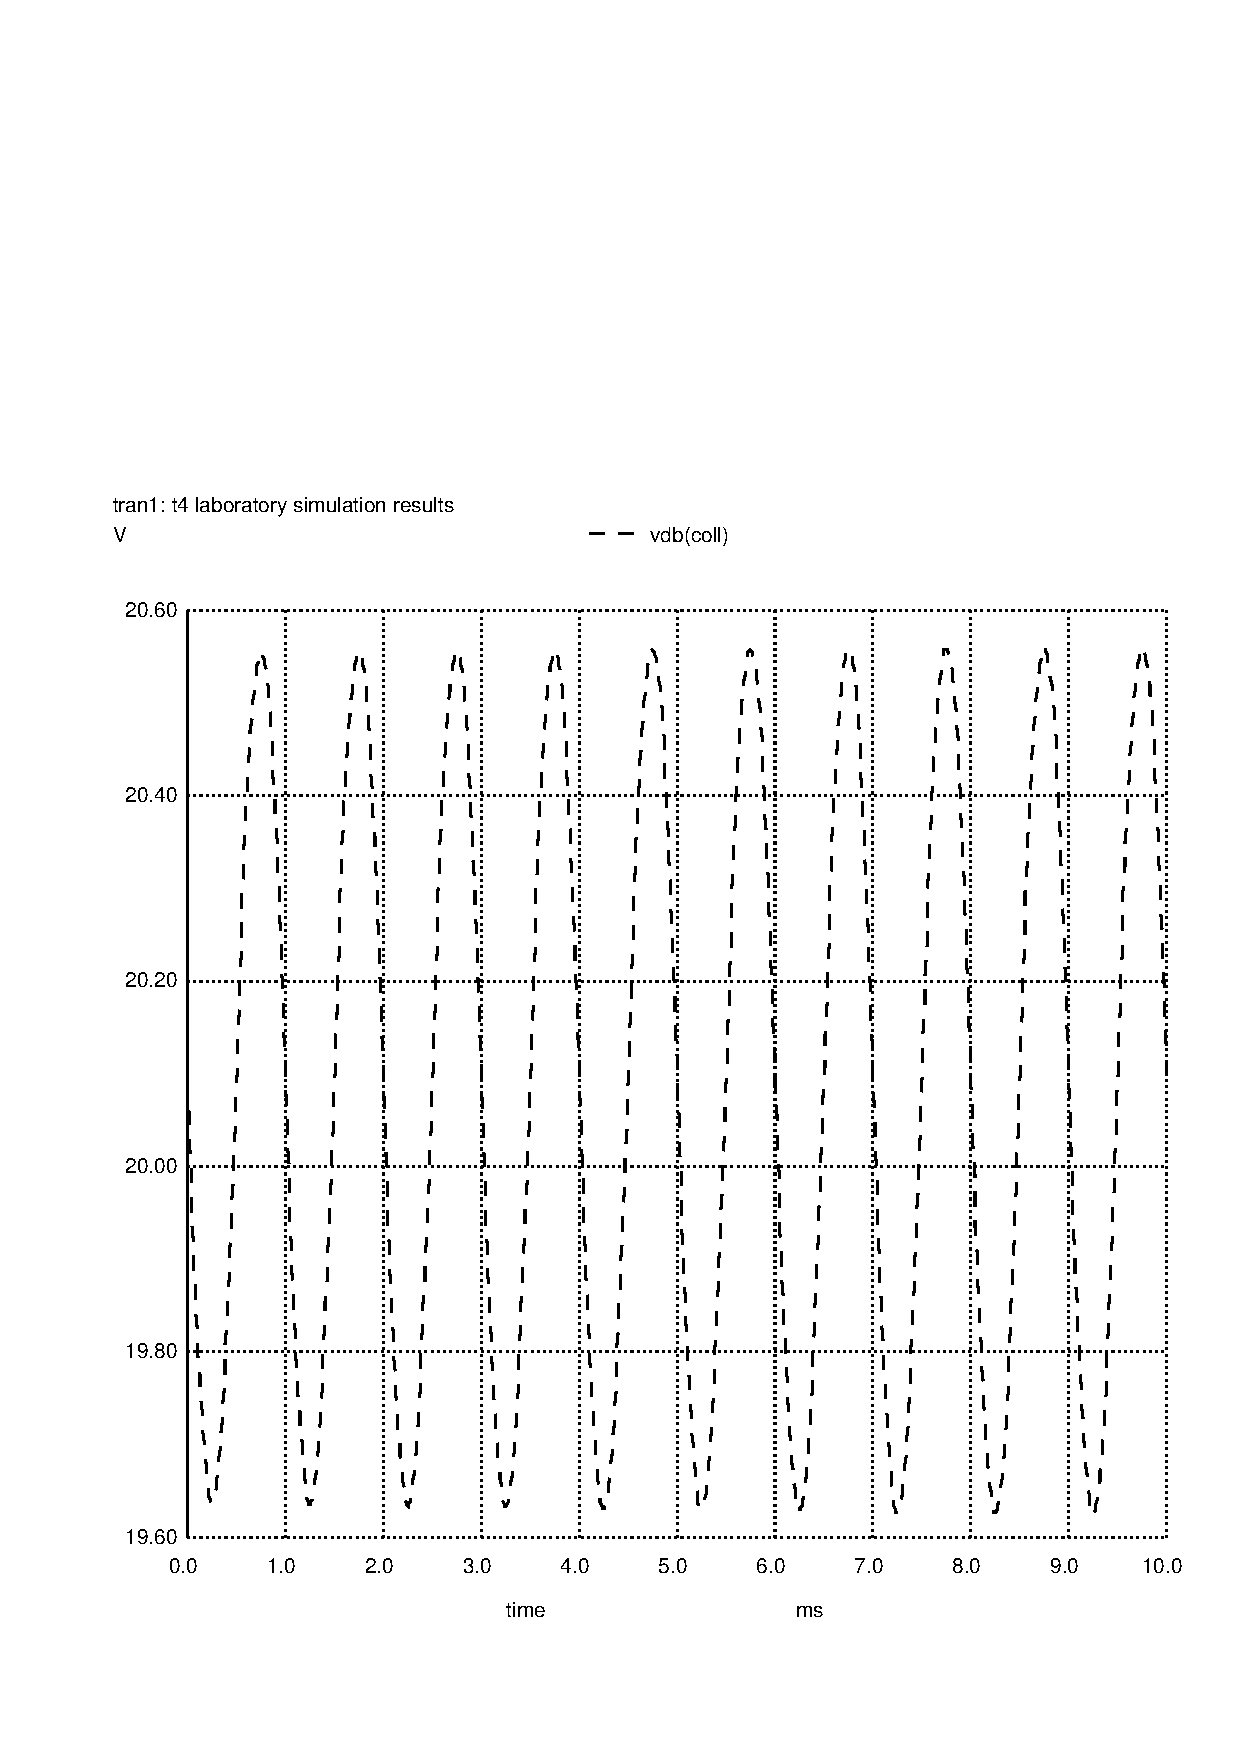
\includegraphics[width=0.4\linewidth]{vo1.pdf}
\caption{LLLLLLLLLLLLLLLLL}
\label{fig:1}
\end{figure}

\begin{figure}[H] \centering
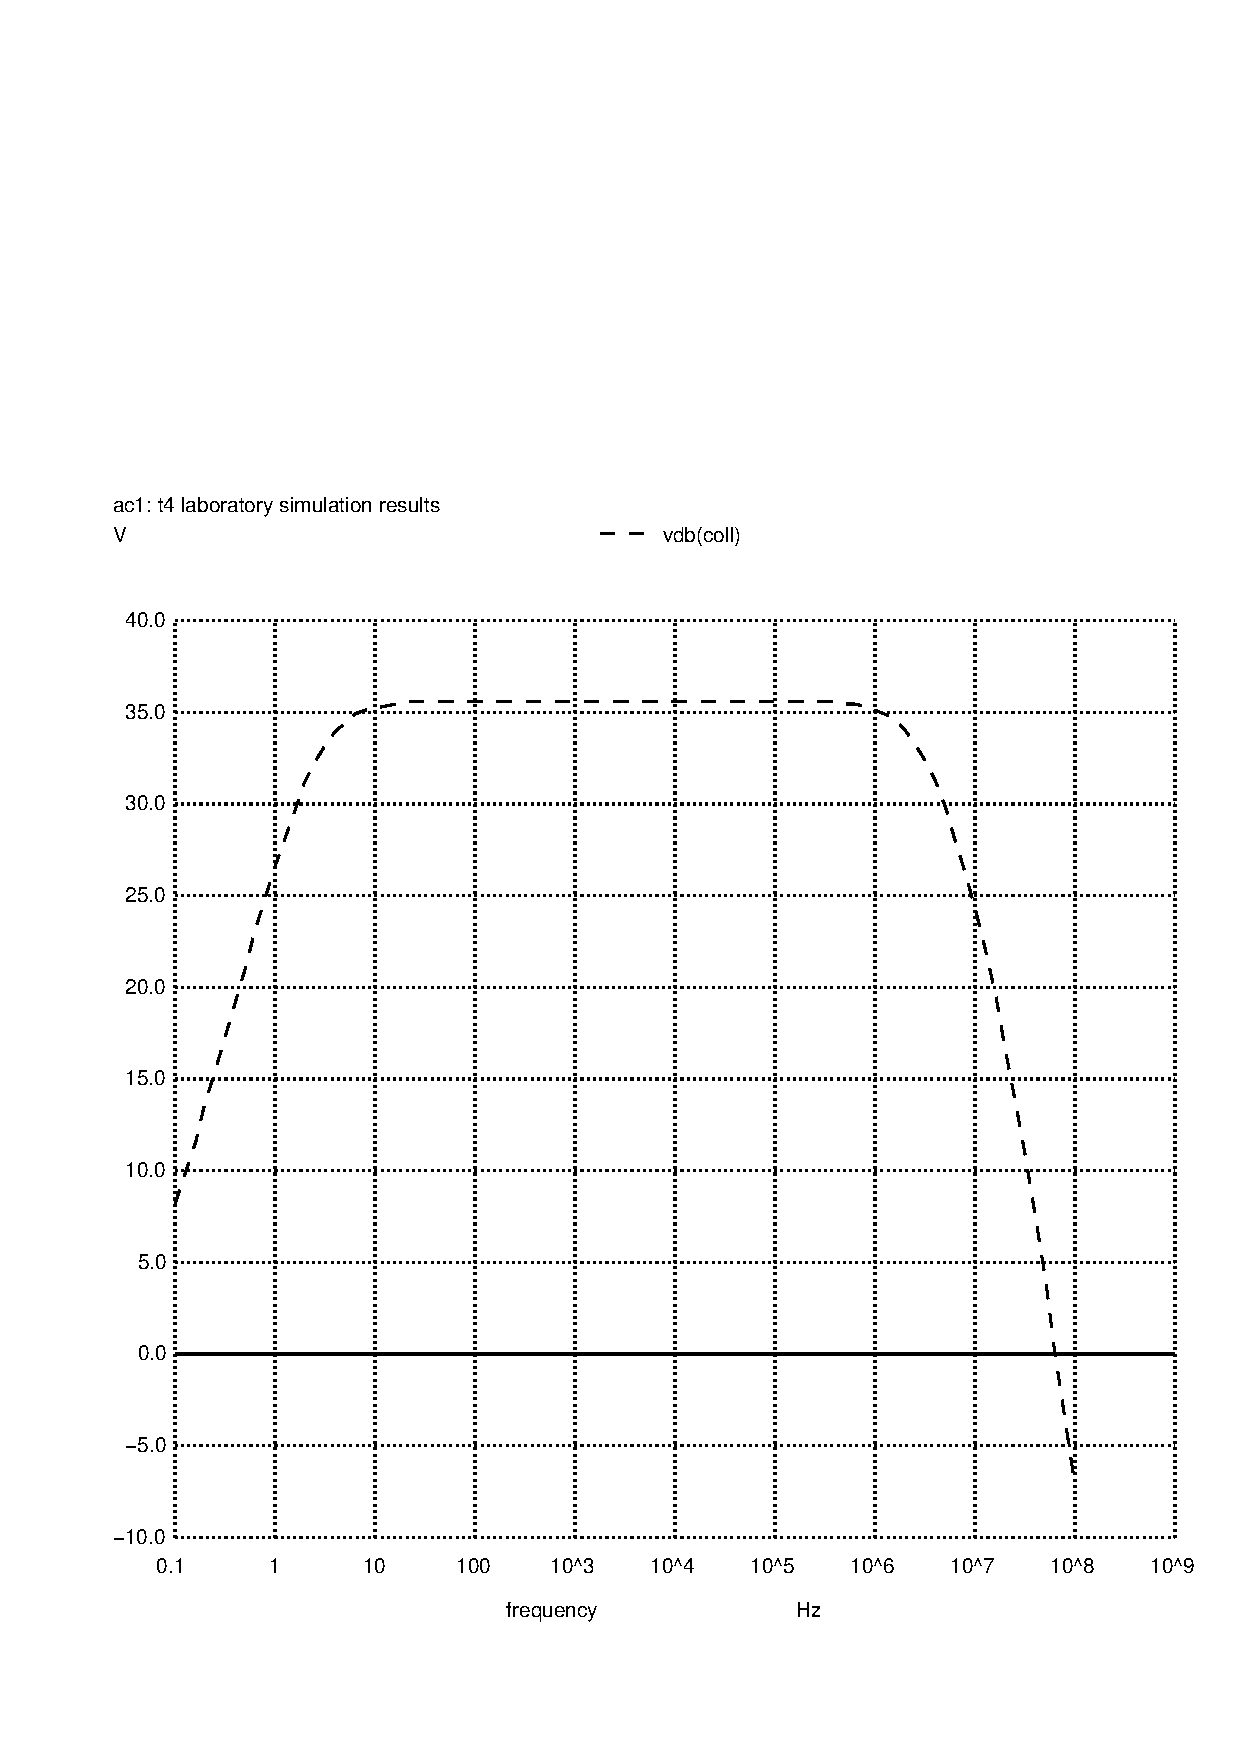
\includegraphics[width=0.4\linewidth]{vo1f.pdf}
\caption{LLLLLLLLLLLLLLLLL}
\label{fig:1}
\end{figure}

\begin{figure}[H] \centering
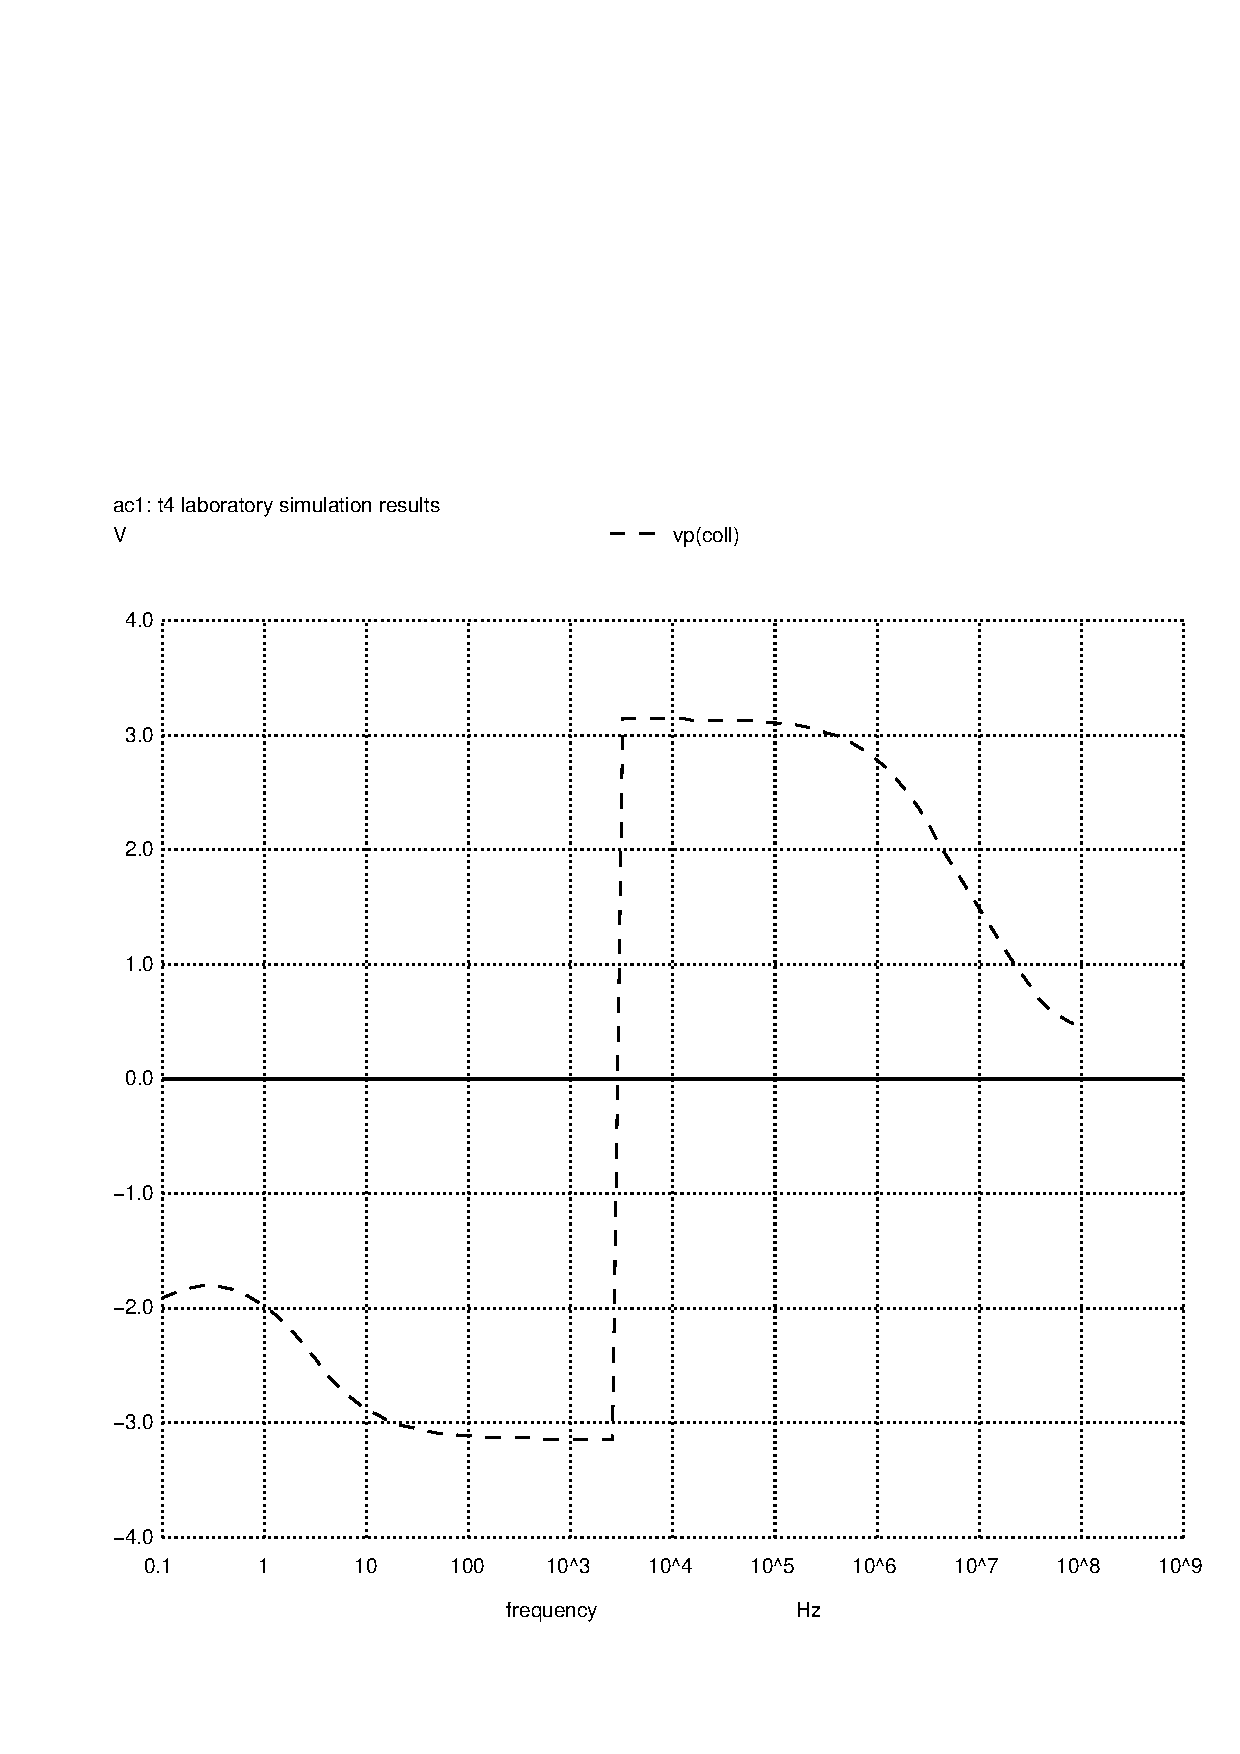
\includegraphics[width=0.4\linewidth]{vo1f2.pdf}
\caption{LLLLLLLLLLLLLLLLL}
\label{fig:1}
\end{figure}

\begin{figure}[H] \centering
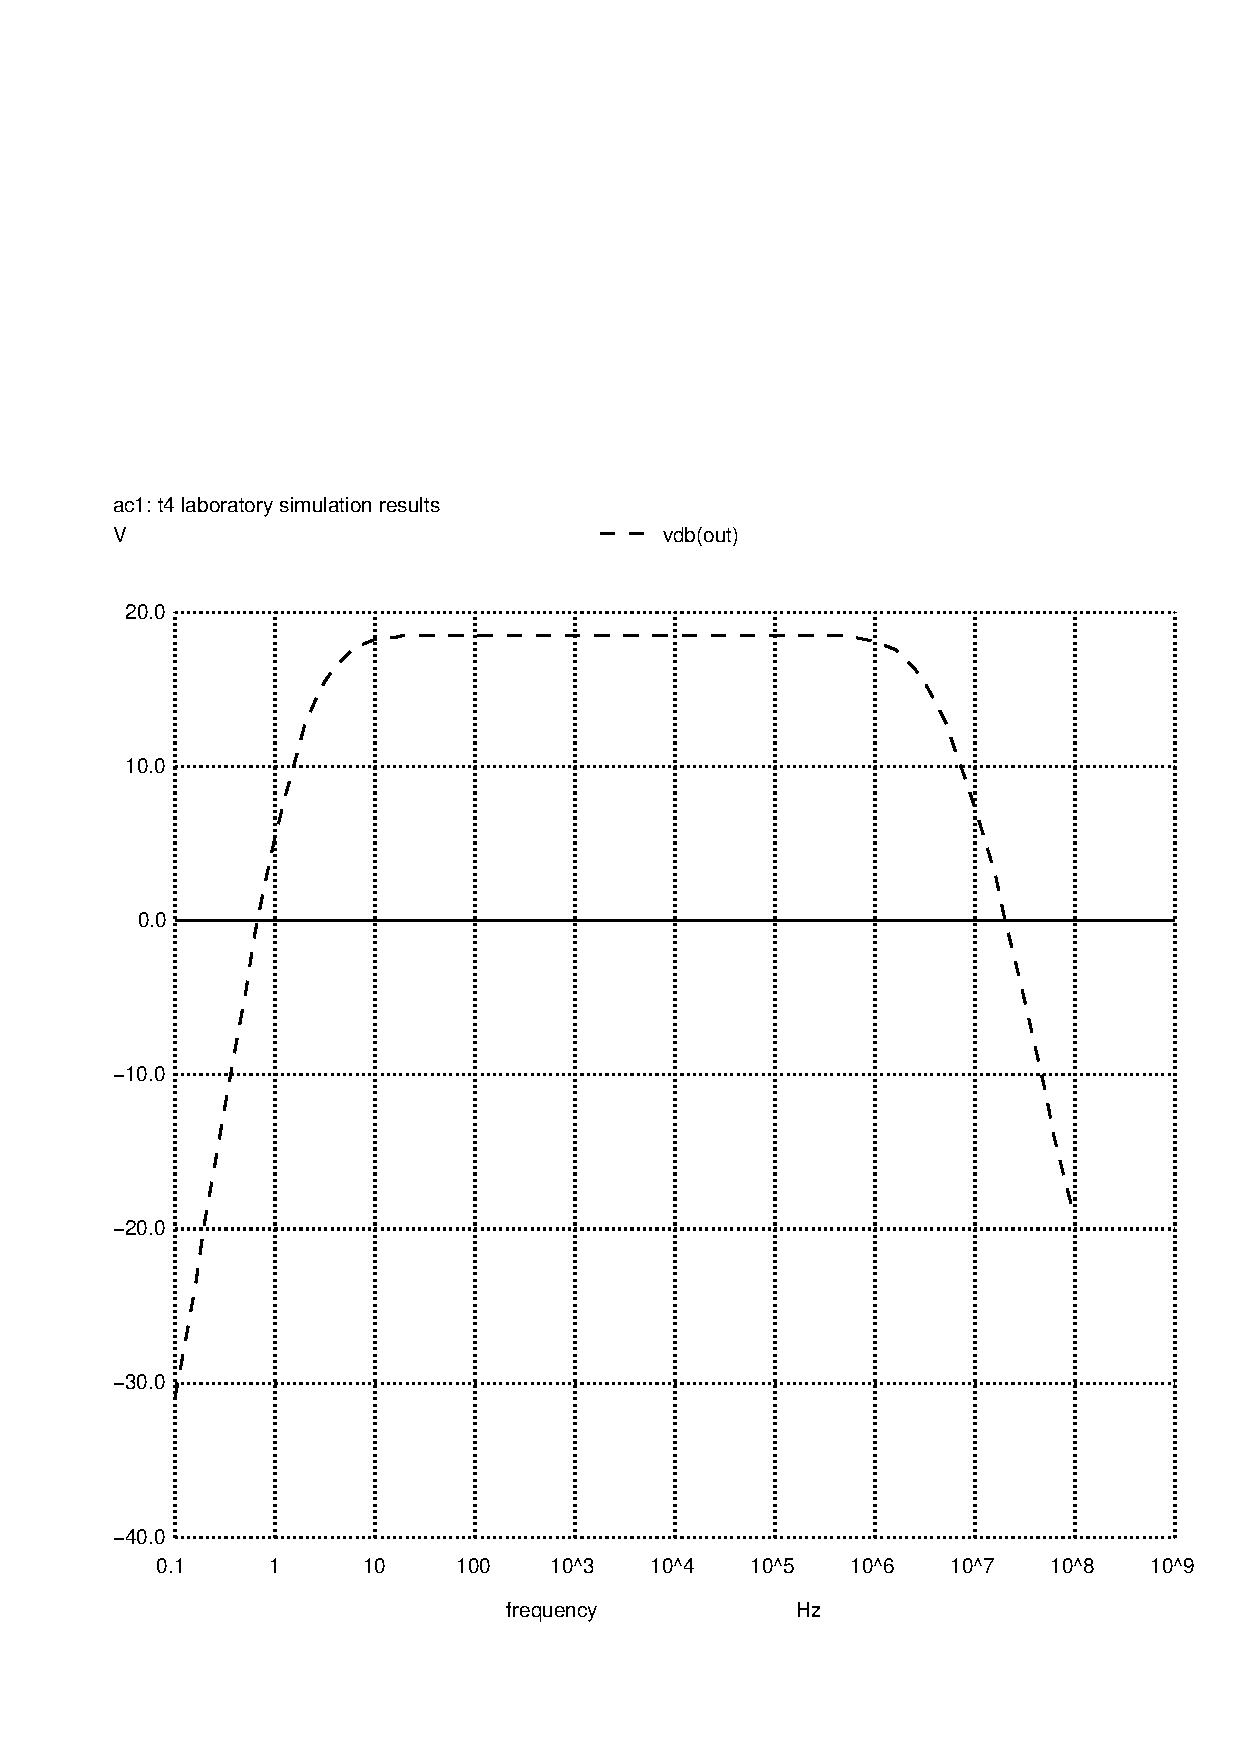
\includegraphics[width=0.4\linewidth]{vo2f.pdf}
\caption{LLLLLLLLLLLLLLLLL}
\label{fig:1}
\end{figure}

\begin{figure}[H] \centering
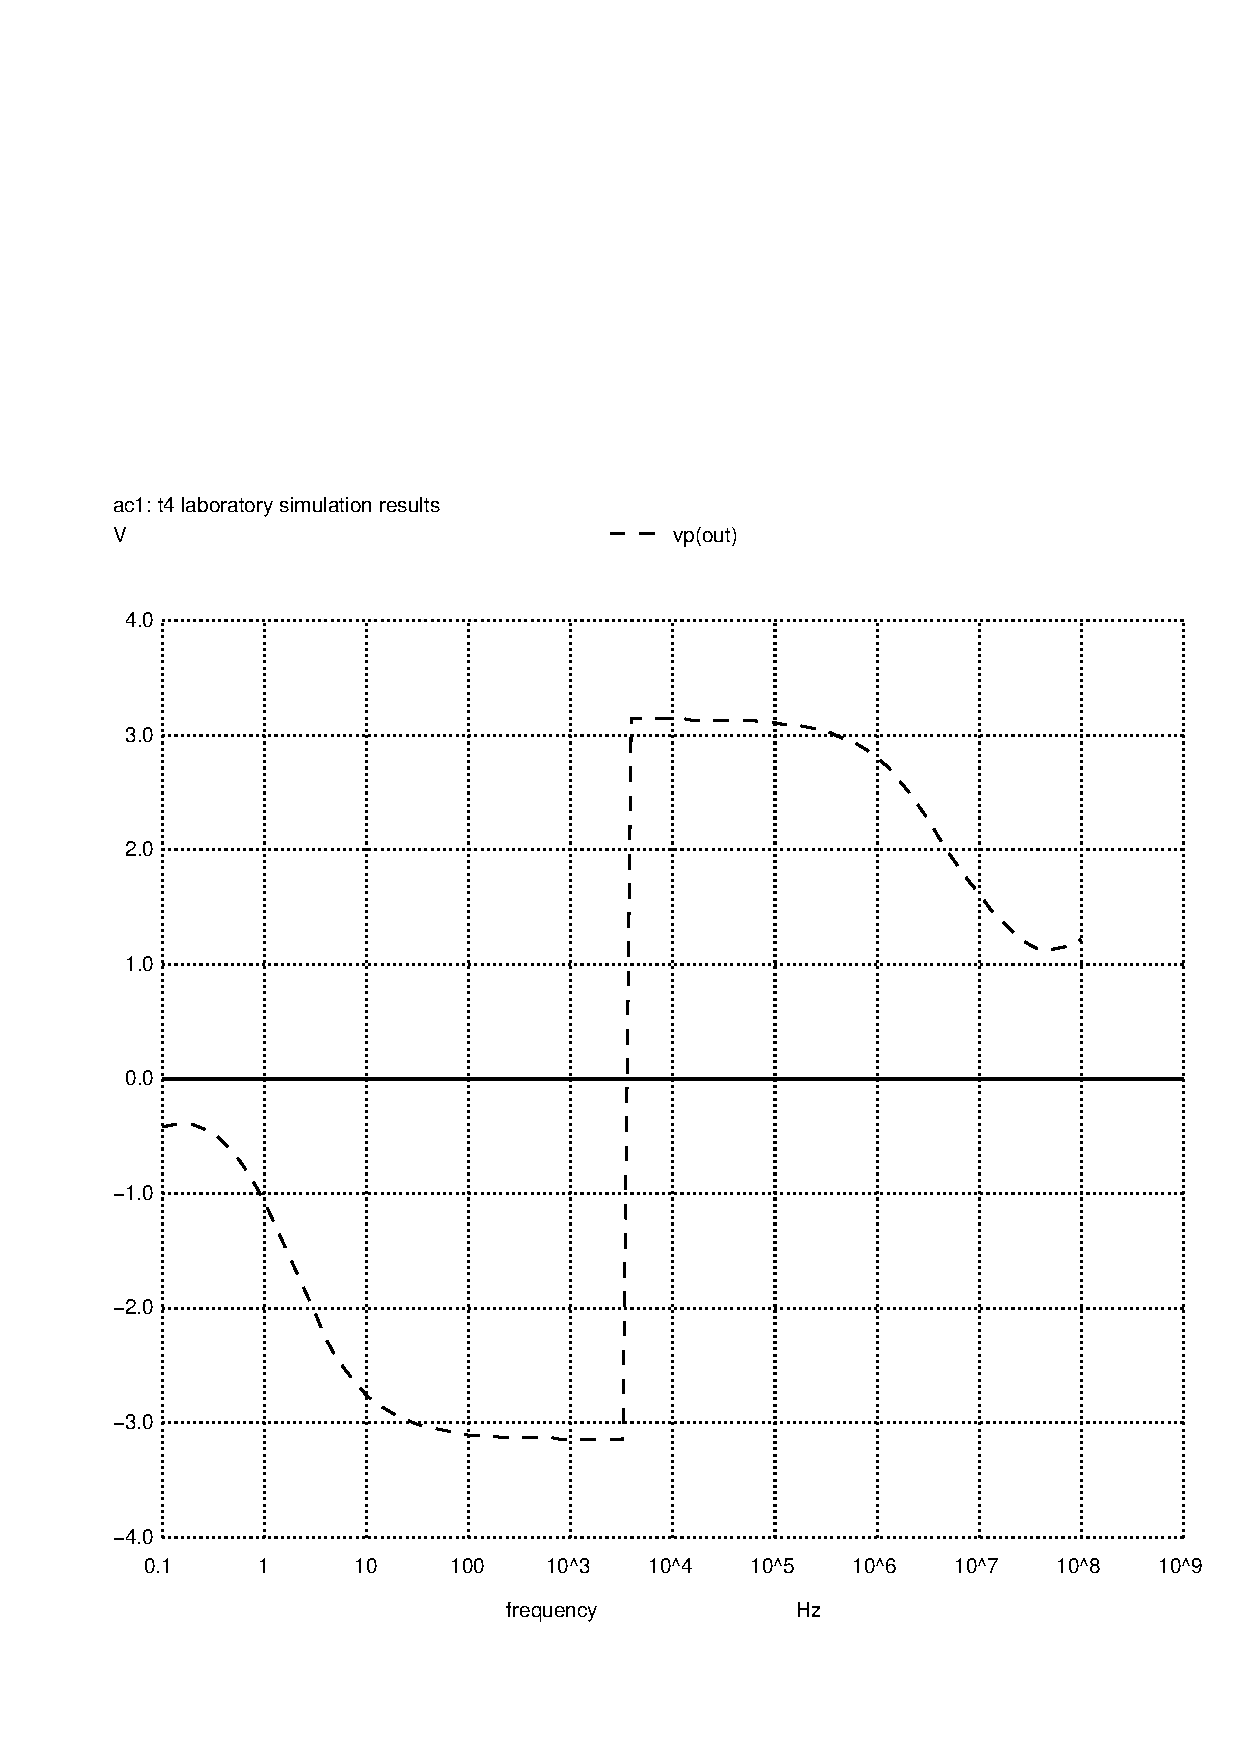
\includegraphics[width=0.4\linewidth]{vo2f2.pdf}
\caption{LLLLLLLLLLLLLLLLL}
\label{fig:1}
\end{figure}
%------------------>>>>>>>>>>>>TABELA EXEMPLO SIDE BY SIDE<<<<<<-------------------------
%\begin{table}[H]
%  \centering
%  \begin{tabular}{|l|r|}
%    \hline    
%    {\bf Name} & {\bf Voltage[V]} \\ \hline
%    \input{../sim/op2_tab}
%  \end{tabular}
%  \begin{tabular}{|l|r|}
%    \hline    
%    {\bf Name} & {\bf Voltage[V]} \\ \hline
%    \input{../mat/Ripple_tab}
%  \end{tabular}
%  \caption{Ripple voltage max$V_4$ - min$V_4$ and the average voltage difference $V_4$ - 12. The values on the right are the theoretical 
%  values for the same voltages in the circuit.}
%  \label{tab2:op}
%\end{table}





